\section{结果与讨论}

\subsection{归一化响应}

按式\eqref{eq:response}计算，输出随 $\theta$ 单调上升，但增幅逐渐减小。图~\ref{fig:step-response} 中两处标记分别对应 $1-\exp(-1)$ 与 $1-\exp(-3)$。在上述假设下，改变 $\tau$ 只缩放时间轴，不改变归一化曲线。

% 路径相对于根目录；图题在图下，标签紧跟图题。
\begin{figure}[htbp]
  \centering
  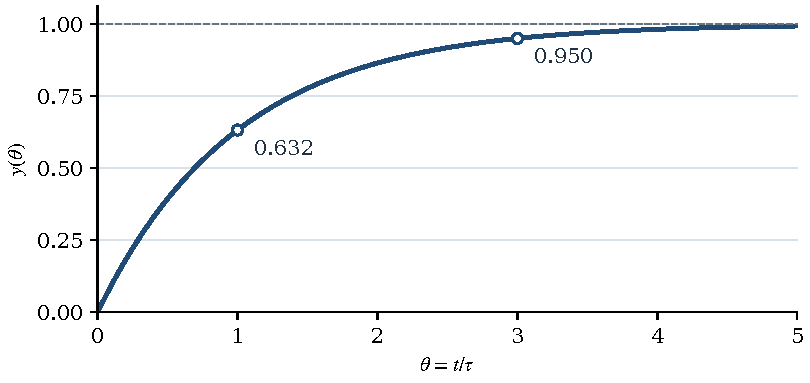
\includegraphics[width=0.76\linewidth]{figures/step-response.pdf}
  \caption{单位阶跃输入下的一阶系统归一化响应}
  \label{fig:step-response}
\end{figure}

\subsection{固定时刻比较}

表~\ref{tab:time-constants} 给出在同一时刻的计算值。$\tau$ 从 \qty{0.5}{\second} 增至 \qty{2.0}{\second} 时，输出从约 $0.982$ 降至 $0.632$。这是因为更大的时间常数对应更小的 $t/\tau$，而不是因为系统稳态增益变小。

% 表题在表上，表注在表底线下；S 列按小数点对齐。
\begin{table}[htbp]
  \centering
  \caption{不同时间常数下的固定时刻响应}
  \label{tab:time-constants}
  \begin{tabular}{@{}l S[table-format=1.1] S[table-format=1.1] S[table-format=1.3]@{}}
    \toprule
    工况 & {$\tau/\unit{\second}$} & {$t/\tau$} & {$y(t)$} \\
    \midrule
    较快 & 0.5 & 4.0 & 0.982 \\
    基准 & 1.0 & 2.0 & 0.865 \\
    较慢 & 2.0 & 1.0 & 0.632 \\
    \bottomrule
    \multicolumn{4}{@{}l@{}}{\zihao{5} 注：取 $t=\qty{2}{\second}$，输出保留三位小数。}
  \end{tabular}
\end{table}
